\documentclass[12pt]{article}
\usepackage[utf8]{inputenc}
\usepackage{graphicx}
\usepackage{hyperref}
\graphicspath{ {./} }
\usepackage[a4paper,width=150mm,top=25mm,bottom=25mm]{geometry}

\title{Testing Policy}
\author{Ctrl Alt Defeat}

\begin{document}
\begin{titlepage}
    \centering



    \vspace{2cm}
    \hrulefill\\
    \vspace{1cm}
    {\Huge\bfseries SRS Documentation v3.0}

    \vspace{1cm}

    {\Large Software Requirements Specification Document for\\Domain Pulse}\\
    \vspace{1cm}
    \hrulefill\\

    \vfill

    {\large Ctrl Alt Defeat}

    \vspace{1cm}

    {\large 2023/07/31}\\
    %    \vspace{1cm}
    %    \vspace{1cm}
    %    
\includegraphics[width=10cm]{../../Images/dpLogo.png}
    %    \vspace{1cm}\\
    %    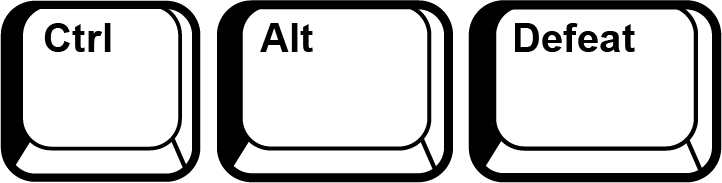
\includegraphics[width=6cm]{../../Images/cadLogo.png}

\end{titlepage}


\tableofcontents
\newpage

\newpage
\section{Quality Requirements Testing}
\subsection{Usability}
Process of Usability Testing:
\begin{itemize}
    \item \textbf{Planning} - The first step in usability testing is to plan what you want to test and how you are going to test it.
    \item \textbf{Recruiting} - The next step is to recruit participants to test the application. The participants should be representative of the target audience of the application but should also be diverse enough to get a wide range of feedback.
    \item \textbf{Testing} - The next step is the actual testing of the application, the way in which we facilitated the testing of the application was as follows:
    \begin{itemize}
        \item We sent all participants of our usability testing a pdf explaining all aspects of navigating to the app and a list of tasks in which they could try. The pdf can be found \href{https://github.com/COS301-SE-2023/Domain-Pulse-A-Sentiment-Analysis-Platform/blob/docs/Demo4Documentation/documentation/Testing%20Policy/Testing_Assistance_Domain_Pulse.pdf}{HERE.}
        \item The participant will access the application in their own time in the environment of their liking and use the application to perform tasks that were suggested on the pdf.
        \item Once the user has completed the testing of the app, a questionaire was then to be filled out by all participants the questionaire can be found \href{https://forms.gle/P6EC4iyg7ZD93LNfA}{HERE.}
    \end{itemize}
    \item \textbf{Feedback implementation} - We collect all data from the questionaire that the testing participants filled out and use this to modify and fix issues accordingly.
\end{itemize}
\begin{itemize}
    \item \textbf{Metrics for usability testing} - The metrics that we used to measure the usability of our application are as follows:
    \begin{itemize}
        \item How insghtful the application is which is computed as an average with 10 being the most insightful and 1 being the least insightful.
        \item The overall rating of the application which is computed as an average with 10 being the best rating and 1 being the worst rating.
        \item The amount of responses regarding how easy the website is to use and navigate ranging from very easy to very diffucult.
        \item The overall sentiment of the responses regarding the application.
    \end{itemize}
\end{itemize}
It is understood that the environment in which the users completed the testing in were all up to the users choice which allows for skewed results in terms of the environment variable not being kept constant and things like noise pollution etc can all have effects on how one would use the app but we belive that this bias of an inconstant environment is neutralised by the adaptability of the app to be used in any environment. NEED TO ADD ONTO REPORT ONCE WE HAVE RESULTS FROM QUESTIONAIRE


\newpage
\subsection{Security}
\subsection{Performance}
\subsection{Scalability}
\subsection{Modifiability}

\newpage
\section{Code Coverage}
Any commit made to a branch causes automated tests to be run on the codebase of that branch, thereafter the code coverage of said branch is calculated.
Any branch being merged via pull request into the development branch (dev) needs to have the coverage of changes to the codebase to match or better the coverage of the development branch.
Furthermore, the coverage of the newly commited code (ie: patch) must match or exceed the coverage percentage of the project.
This ensures that the coverage of the codebase is never decreasing, and that sufficient testing is being done on the codebase.
Furthermore any time the development branch is merged into the master branch, the coverage of the development branch must match or be higher than that of the master branch, ensuring an increasing coverage and sufficient testing.
\begin{itemize}
    \item A code coverage report is included in the below image:
    \item A link to our code cov profile can be found \href{https://codecov.io/gh/COS301-SE-2023/Domain-Pulse-A-Sentiment-Analysis-Platform}{HERE.}
\end{itemize}
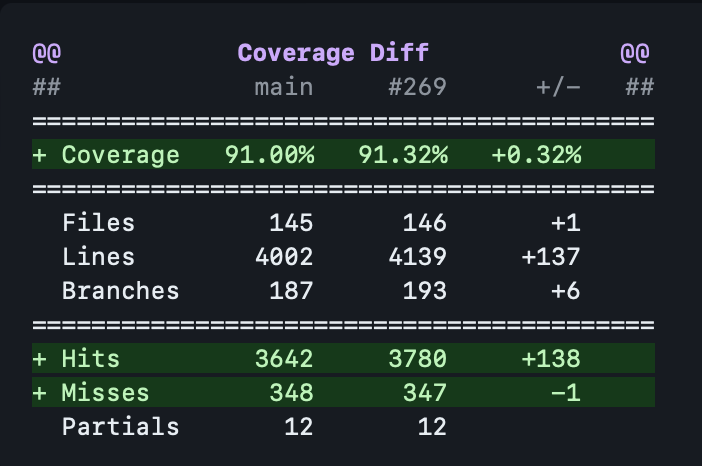
\includegraphics[width=\textwidth]{codecovReport.png}

\newpage
\section{Types of testing}
\begin{itemize}
    \item \textbf{Unit testing} - Unit testing is when the smallest parts of the application which are known as units are tested to ensure that the correct operation occurs. An example of Unit tests and integration tests can be found in any file ending in "spec.ts" for frontend and an example is given \href {https://github.com/COS301-SE-2023/Domain-Pulse-A-Sentiment-Analysis-Platform/blob/dev/frontend/src/app/main/main.component.spec.ts}{HERE.}
    \item \textbf{Integration Testing} - Integration testing is when separate components are tested together to ensure the correct operation of these components occur. Integration tests can be mocked or unmocked, mocked tests are when the data used in the tests are not pulled in from an external API or database but rather mocked data is used to simulate the data that would be pulled in from an external API or database. Unmocked tests are when the data used in the tests are pulled in from an external API or database.
    \item \textbf{E2E Testing} - End to end testing is when the application is tested as a whole to ensure that the application is working as expected from the user interface level all the way through the application to the database level and checks all the integration between these componets work as expected. Examples of E2E tests can be found in any file ending in a ".cy.ts" for frontend and an example is given \href {https://github.com/COS301-SE-2023/Domain-Pulse-A-Sentiment-Analysis-Platform/blob/main/frontend/cypress/e2e/accountsManage.cy.ts}{HERE.}
\end{itemize}
\newpage
\section{Choice of testing tools/frameworks}
\subsection{Frontend Testing}
For our frontend testing frameworks and tools we decided to use the following:
\begin{itemize}
    \item \textbf{Karma and Jasmine} - Jasmine is the testing framework that is used to write actual tests and are typed in Javascript, Karma is the test runner that executes the tests. Karma is run from a CLI(Command Line Interface) and it will open up a browser window and run the tests in that browser. Karma will then report the results of the tests back to the CLI and can be used to generate a coverage report. Karma and Jasmine are recommended by Angular which is what our frontend is primarily built upon and they are the most popular testing frameworks for Angular applications. The advantages of using Karma and Jasmine over other testing frameworks is that they are easy to set up and use, they are well documented and they are popular amongst Angular developers which means there is a extensive amount of resources available online for help if need be.
    \item \textbf{Cypress} - Cypress is a testing framework that is used to write end to end tests which are tests that try and simulate a user using the application. End to end tests are needed to ensure that the application is working exactly as expected from the user interface level all the way through the application to the database level and checks all the integration between these componets work as expected. Cypress runs in a browser which makes it easy to setup and follow the tests as they excute in the browser. Cypress is documented well with a thriving community which allows for easy access to information if any problems arise.
\end{itemize}

\subsection{Backend Testing}
For our backend testing framework and tools we decided to use the following:
\begin{itemize}
    \item \textbf{Django built in testing module} - Django has a built in testing module which allows for the testing of Django applications, this is yet another reason why we decided to use django as it has amazing functionality out of the box. The django testing module allows for extensive testing of the application. The advantages of using django testing framework over an external framework is that one is already used to the syntax of django since our backend is primarily built on django and hence saves valuable time trying to learn syntax of another backend testing framework. Django allows for fast pace development which is much needed in certain situations such as in ours when following an agile development strategy. Django testing framework is also well documented and has a large community which allows for easy access to information if any problems arise and help is needed.
\end{itemize}

\subsection{Github Actions and workflows}
Github actions were used to aid in the automatic testing and generating of code coverage reports for our application. Github actions are workflows that are activated by certain events such as a merge, push or pull to certain branches of the repository. The workflows are defined in a yaml file and are run on a virtual machine hosted by github, Github actions ensure that all tests pass before a branch is merged into main/master. The workflows that we have defined are as follows:
\begin{itemize}
    \item backend build
    \item frontend build
    \item coverage report
    \item automatic deployment
    \item automatic testing
\end{itemize}

\end{document}